\documentclass[../main.tex]{subfiles}

\begin{document}

%%%%%%%%%%%%%%%%%%%%%%%%%%%%%%%%%%%%%%%%%%%%%%%%%%%%%%%
%   New Chapter                                       %
%%%%%%%%%%%%%%%%%%%%%%%%%%%%%%%%%%%%%%%%%%%%%%%%%%%%%%%

\chapter{Sparse Coding}
In this and the next chapter, we will take a classical view on representing data which is inspired from signal processing. This chapter will have less to do with machine learning but more just about ideas to represent data/signals, specifically in a sparse way, while in the next chapter we will take about how to learn these representations. Our discussion will start by requiring orthogonality for the basis with two widely used examples: Fourier basis and wavelet basis. We will then compare them with PCA in terms of data compression to put some connection back to things we have already covered. Image compression will also be briefly discussed. Then we go beyond the orthonormal basis to a new family of coding that exploits redundancy in representation to benefit sparsity. The discussion is followed by how to construct such dictionaries as well as how to reconstruct the signal based on that dictionary.
\section{Sparse Coding}
A basic observation in signal processing is that signals can be represented in different ways. For any given signal, we actually can find infinite number of possible representations, each of which usually captures different characteristics for the signal. For example, as shown in Figure \ref{fig_9_1}, a periodic signal in time domain can usually be represented in a much simpler way in terms of Fourier series. These (simple) representations, usually reveal a lot about the signals giving some useful insight and also open up other possibilities like data compression or finding better representations. 
\begin{figure}[h] 
	\centering 
	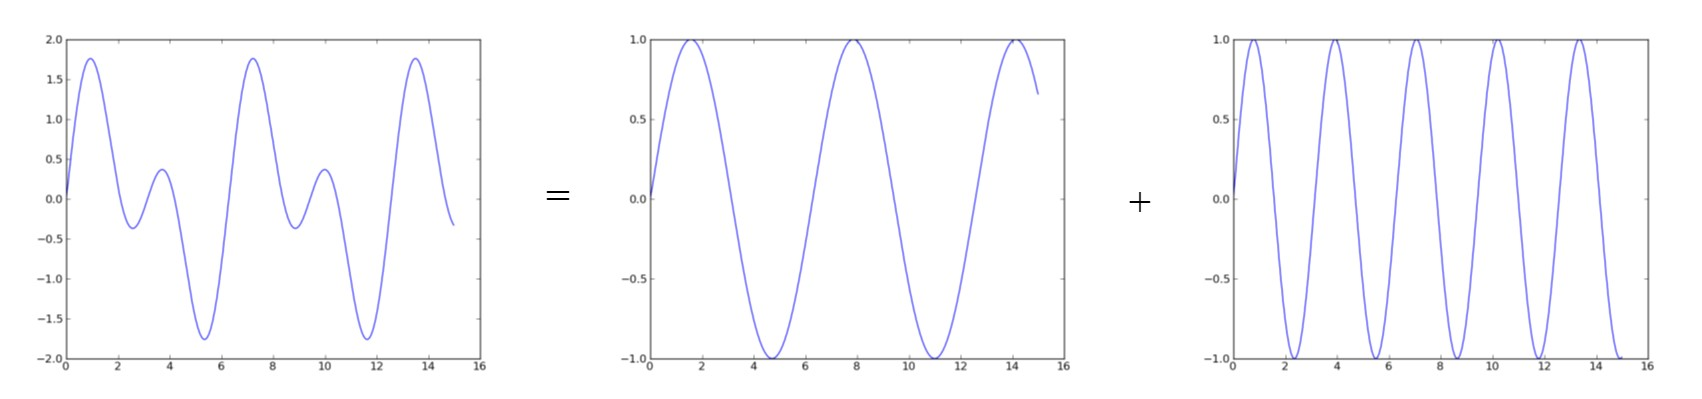
\includegraphics[width=12cm]{fig_9_1.jpg} 
	\caption{Periodic signals usually have a simple representation in Fourier basis.}\label{fig_9_1}
\end{figure}
\par Another general observation that motivates sparse coding is that natural signals often allow for sparse representation. For sparsity, we mean that in the representations many coefficients vanish ($\approx 0$) with only a few ones are non-zero. This is justified by the assumption on the regularities of signals. Just like signals for human speaking should not be any time series but forms a particularly small and highly-structured subset of all acoustic signals. To reveal the sparsity, we need to find a suitable dictionary of atoms $\mathcal{U}=\{{\bf u}_1,\dots,{\bf u}_L\}$, which can be predefined or learned from data (will be discussed in the next chapter). The original signal should have an accurate representation in span($\mathcal{U}$) with only a few atoms.
\subsection{Signal Compression}
A very simple setup we can think of as a start is the following. Given the original signal ${\bf x}\in \mathbb{R}^D$ and orthonormal matrix ${\bf U}=({\bf u}_1,\dots,{\bf u}_D)$ (the dictionary), we can re-represent ${\bf x}$ in a different basis by compute a linear transformation:
\begin{equation*}
{\bf z}=\underbrace{{\bf U}^T}_{D\times D}\cdot {\bf x}.
\end{equation*}
As a direct consequence of orthogonality, the energy/length is preserved after the transformation in the sense that
\begin{equation*}
\|{\bf U}^T{\bf x}\|^2 = \|{\bf x}\|^2.
\end{equation*}
Note that the preservation of length implies the preservation of angles. As a rather intuitive explanation, every angle in a triangle remains the same after orthonormal transformation (due to the fact that edges stay the same). At this point, there is no loss of information since we can reconstruct ${\bf x}$ from ${\bf z}$ by ${\bf x}={\bf Uz}$. To force sparsity, we truncate ``small'' values of ${\bf z}\Longrightarrow\hat{\bf z}$. Specifically, we encode only $K\ll D$ non-zeros values. This can be done by either only keeping the $K$ largest coefficients or employing a threshold $\epsilon$:
\begin{equation*}
\hat{z}_d=\begin{cases}
0 &\ {\rm if}\ |z_d|<\epsilon\\
z_d&\ {\rm otherwise}
\end{cases},
\end{equation*}
which is preferred since this let the data ``speak'' about how sparse should the representation be. For reconstruction, we can simple apply an inverse transform given by
\begin{equation*}
\hat{\bf x}={\bf U}\hat{\bf z}\quad{\rm as}\ {\bf U}^T={\bf U}^{-1}.
\end{equation*}
Here we benefit from the choice of orthonormal basis for the efficient inversion. If the reconstruction error is low, then we have found a sparse representation for ${\bf x}$. To evaluate the reconstruction error, first recall that given ${\bf x}$ and orthonormal basis $\{{\bf u}_1,\dots,{\bf u}_D\}$ (columns of ${\bf U}$), ${\bf x}$ can be decomposed in the form of
\begin{equation*}
{\bf x}=\sum_{d=1}^{D}z_d({\bf x})\cdot {\bf u}_d,\quad z_d({\bf x}):=\langle {\bf x,u}_d\rangle.
\end{equation*}
For sparsification, we keep only a $K$-subset $\sigma$ of basis functions:
\begin{equation*}
\hat{\bf x}=\sum_{d\in \sigma}z_d({\bf x})\cdot {\bf u}_d.
\end{equation*}
This gives the reconstruction error
\begin{equation*}
\|{\bf x}-\hat{\bf x}\|^2=\left\|\sum_{d\notin \sigma}\langle {\bf x,u}_d\rangle \cdot {\bf u}_d \right\|^2 = \sum_{d\notin \sigma}\|\langle {\bf x,u}_d\rangle \cdot {\bf u}_d\|^2 = \sum_{d\notin \sigma}\langle {\bf x,u}_d\rangle^2.
\end{equation*}
This shows that how much energy is lost in thresholding/selecting can be easily computed. Keep in mind that we are not trying to find a sparse representation for a single signal but for a class of signals, say all natural acoustic signals. We want a dictionary works for a whole range of signals, in which these signals are sparsely representable. 
\subsection{Sparse Coding with Fourier Basis and Wavelet Basis}
Now we introduce 2 examples of such orthonormal basis for 1-D signal processing, namely the Discrete Fourier Transform (DFT) and the Discrete Wavelet Transform (DWT). Take the signal shown in Figure \ref{fig_9_2} for an example.
\begin{figure}[h] 
	\centering 
	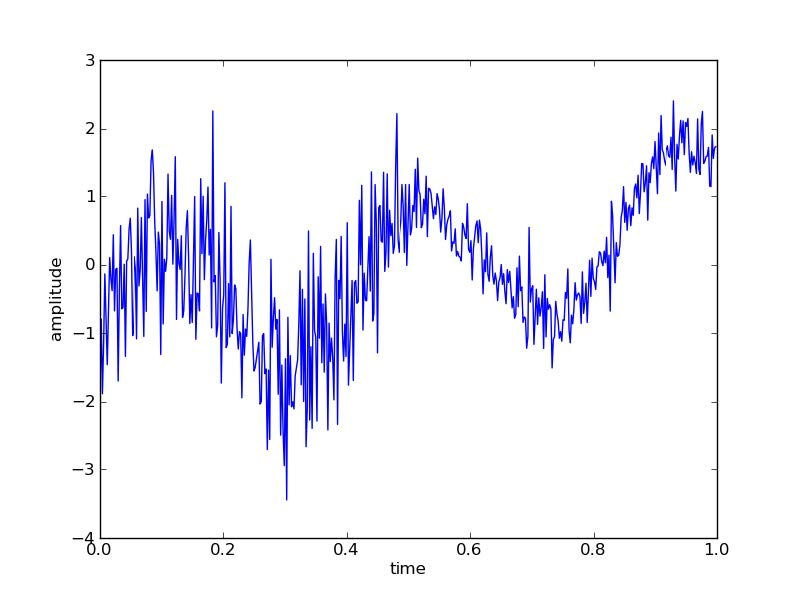
\includegraphics[width=8cm]{fig_9_2.jpg} 
	\caption{A sample signal.}\label{fig_9_2}
\end{figure}
\par We can see a trend with some high frequency noise. If we perform DFT (${\bf z}={\bf U}^T{\bf x}$) who has orthonormal basis in the form of sine functions with different frequencies and plot its spectrum (left of Figure \ref{fig_9_3}) we see that the energy concentrates in the low-frequency part. If we perform an $\epsilon$-thresholding (right of Figure \ref{fig_9_3}) and reconstruct the signal, we get a smooth signal without noise (Figure \ref{fig_9_4}), which can be regarded as being applied with a low-pass filter. Although at the boundaries, the reconstructed signal has some weird behaviors (because DFT assumes periodic signals), in the middle it covers the trend. Since we only keep $3\%$ of the Fourier coefficients, the signal is compressed by $97\%$. The high signal frequencies have small amplitudes in spectrum and therefore are suppressed. In this case, the things we have thrown away could probably be considered as noise, but there might be some useful information in some cases.
\begin{figure}[h] 
	\centering 
	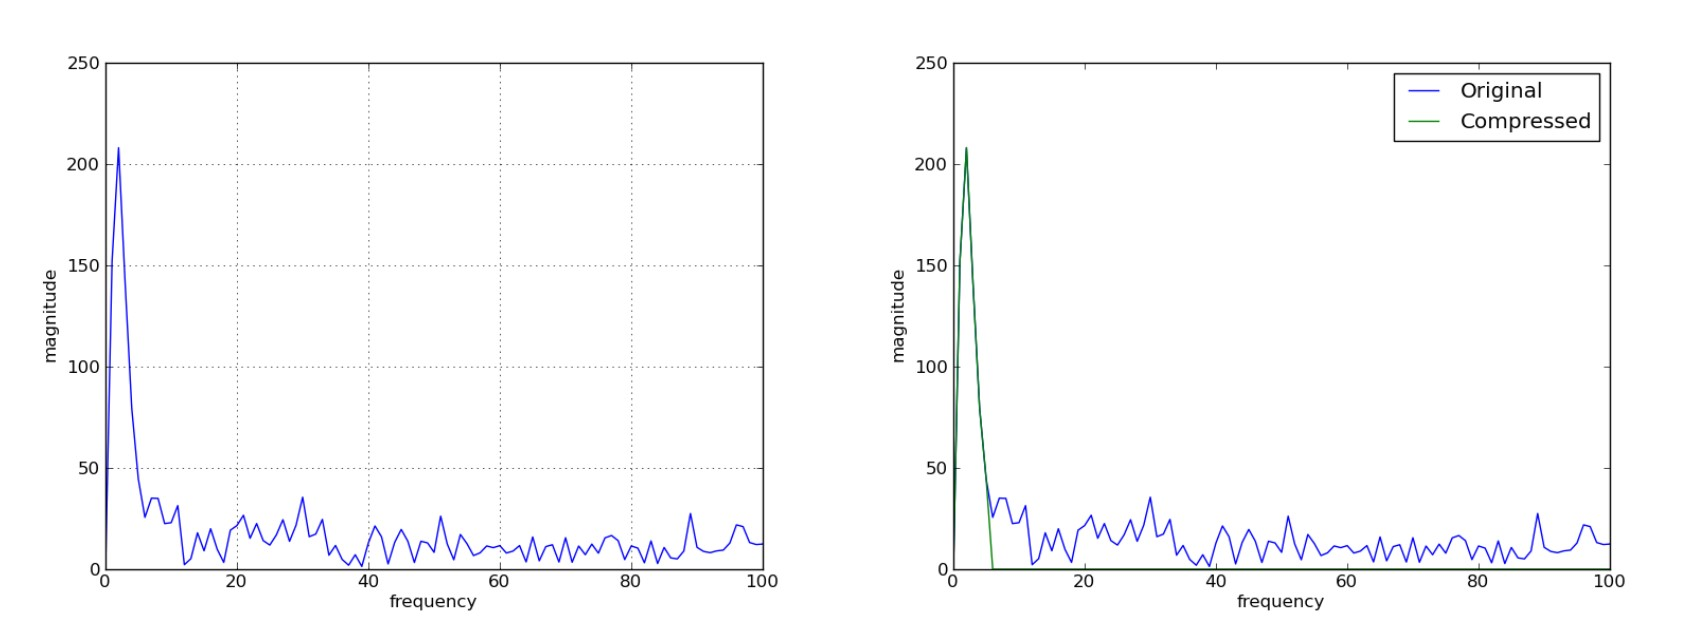
\includegraphics[width=12cm]{fig_9_3.jpg} 
	\caption{Left: Fourier spectrum of signal in Figure \ref{fig_9_2}. Right: retaining $3\%$ of the coefficients $\hat{\bf z}$.}\label{fig_9_3}
\end{figure}
\begin{figure}[h] 
	\centering 
	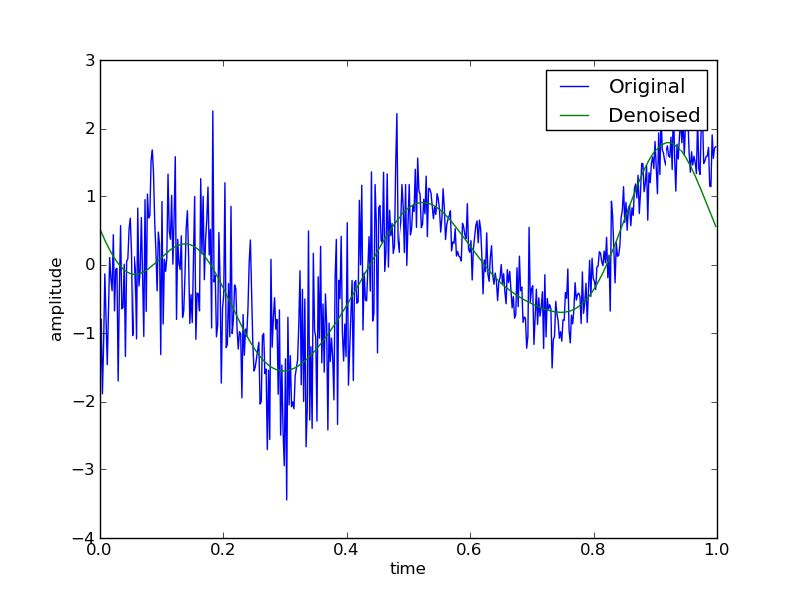
\includegraphics[width=9cm]{fig_9_4.jpg} 
	\caption{Reconstructed signal with DFT: $\hat{\bf x}={\bf U}\hat{\bf z}$ (Denoised).}\label{fig_9_4}
\end{figure}
\par However, is Fourier basis the final answer for all potentially sparse signals? Consider the another example shown in the left part of Figure \ref{fig_9_5}, which shows stronger localized properties than the last one. The denoised signal with DFT is shown in the right part, where it is clear that DFT fails completely.
\begin{figure}[h] 
	\centering 
	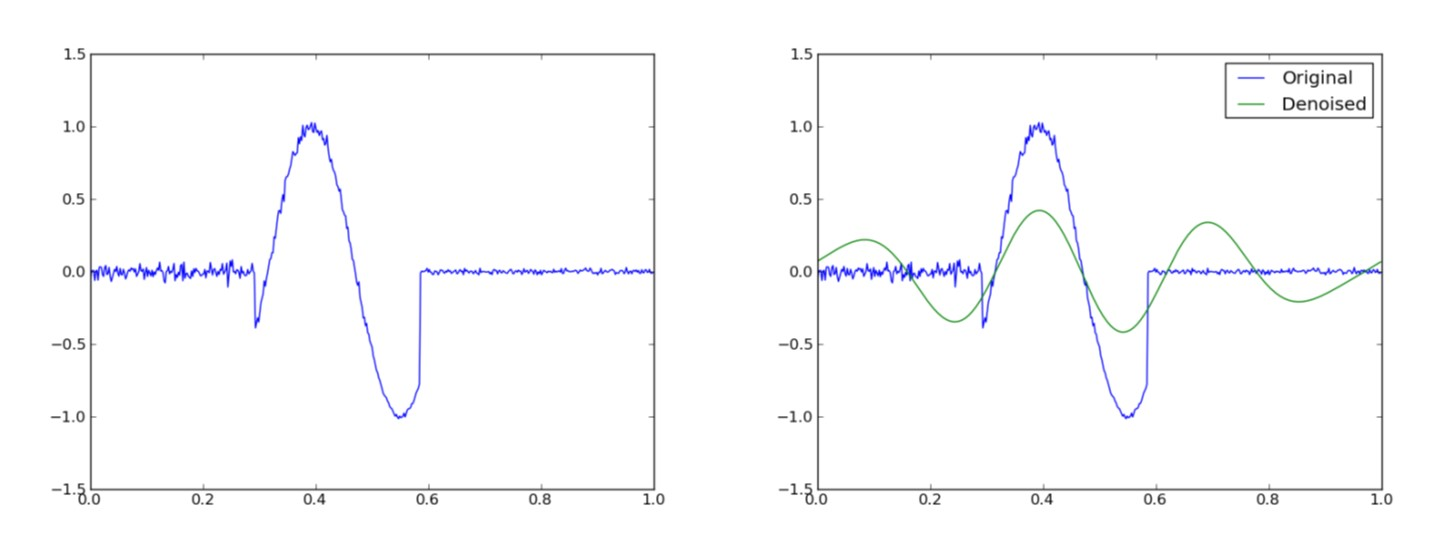
\includegraphics[width=12cm]{fig_9_5.jpg} 
	\caption{Left: a signal fail to be described with DFT. Right: the reconstruction of DFT.}\label{fig_9_5}
\end{figure}
\begin{figure}[h] 
	\centering 
	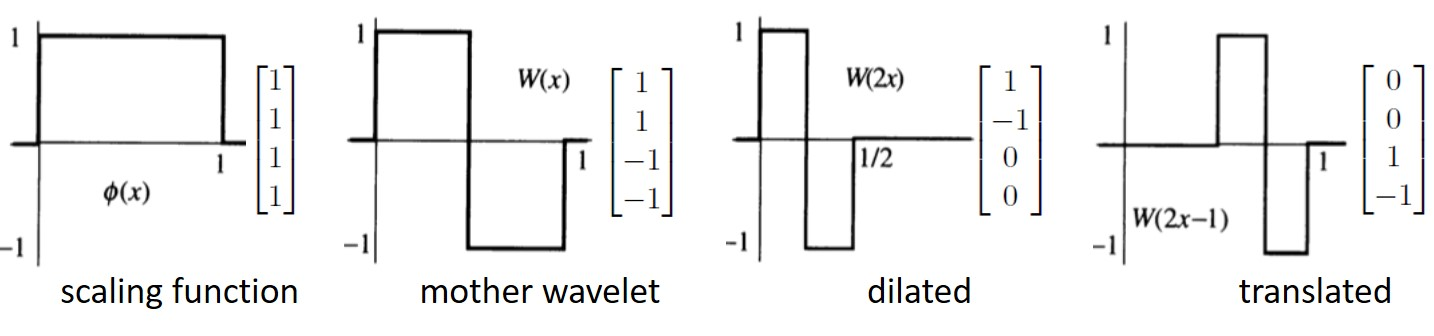
\includegraphics[width=12.5cm]{fig_9_6.jpg} 
	\caption{4-dimension Haar wavelets.}\label{fig_9_6}
\end{figure}
\par Here another important family of orthonormal basis comes into play for these local cases, the wavelets. Take the 4-dimension Haar wavelets as an example (Figure \ref{fig_9_6}). Haar wavelets construct basis consisting of a scaling function (averaging), a mother wavelet that detects changes by contrasting the first and the second half, and some dilated and/or translated mother wavelet. Note that they need to be normalized to form an orthonormal basis. For $D=4$ we get the following orthonormal matrix
\begin{equation*}
{\bf U}=\frac{1}{2}\begin{pmatrix}
1&1&\sqrt{2}&0\\
1&1&-\sqrt{2}&0\\
1&-1&0&\sqrt{2}\\
1&-1&0&-\sqrt{2}
\end{pmatrix}.
\end{equation*}
For $D=8$ we have
\begin{equation*}
{\bf U}=\frac{1}{2}\begin{pmatrix}
1&1&\sqrt{2}&0&2&0&0&0\\
1&1&\sqrt{2}&0&-2&0&0&0\\
1&1&-\sqrt{2}&0&0&2&0&0\\
1&1&-\sqrt{2}&0&0&-2&0&0\\
1&-1&0&\sqrt{2}&0&0&2&0\\
1&-1&0&\sqrt{2}&0&0&-2&0\\
1&-1&0&-\sqrt{2}&0&0&0&2\\
1&-1&0&-\sqrt{2}&0&0&0&-2
\end{pmatrix}.
\end{equation*}
Actually for $D=2^n$ we can keep doing dilation and translation with normalization to form the Haar wavelets. Wavelets can be regarded as little finite supported local time domain filters, and can take other shape with basis generated also by dilation and translation (Figure \ref{fig_9_7}).
\begin{figure}[h] 
	\centering 
	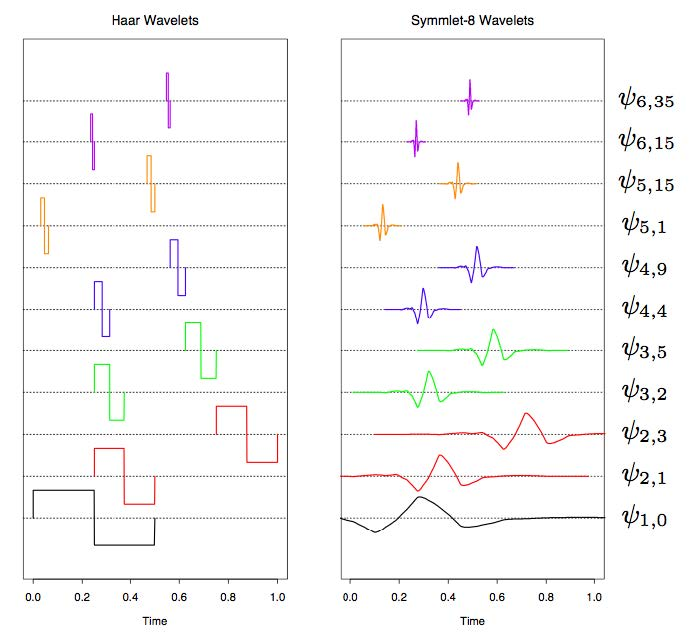
\includegraphics[width=8cm]{fig_9_7.jpg} 
	\caption{Other wavelets.}\label{fig_9_7}
\end{figure}
Using DWT (left of Figure \ref{fig_9_8}) we can construct a denoised localized signal. Also if we apply DWT to the signal in Figure \ref{fig_9_2} we get the right part of Figure \ref{fig_9_8}. Although the reconstruction is not as smooth as the one produced by DFT, it is still good. The pulses appears because of the localized property of wavelet since if something is strong enough locally, wavelets will think there is something interesting happening and captures that. 
\begin{figure}[h] 
	\centering 
	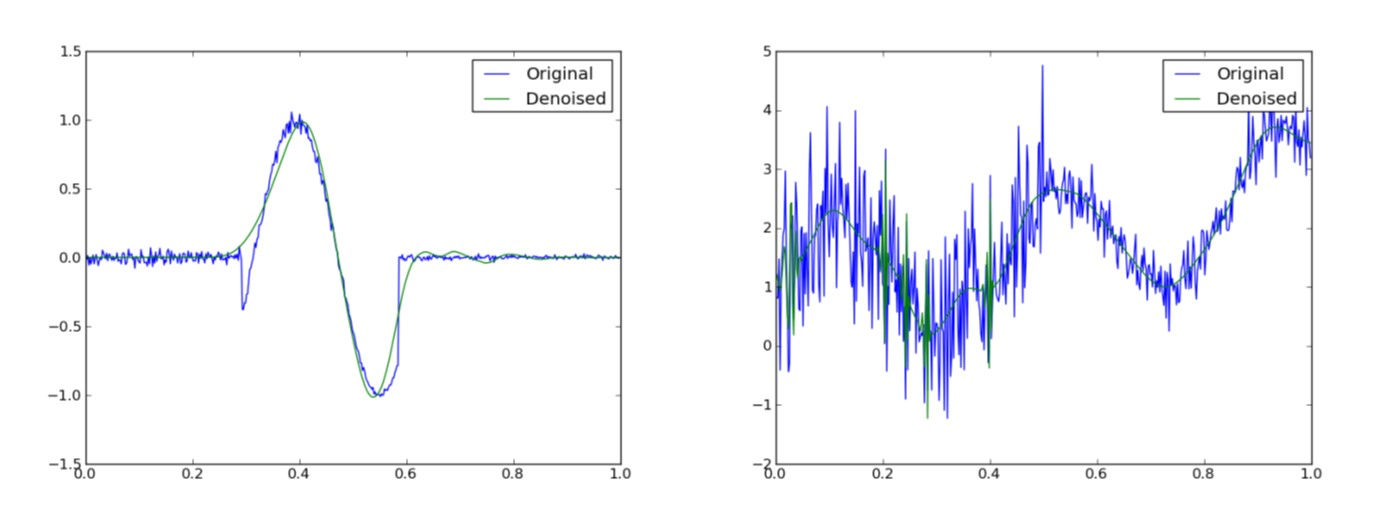
\includegraphics[width=12cm]{fig_9_8.jpg} 
	\caption{Left: DWT for localized signal. Right: DWT for signal in Figure \ref{fig_9_2}.}\label{fig_9_8}
\end{figure}
\par There does not exist a choice of a transform that is better than all other choices. It depends on the signal type. The Fourier basis has global support and is good for ``sine-like'' signals, while is poor for localized signals. The wavelet basis, on the contrast, has local support and is good for localized signals while is poor for non-banishing signals. In practice, it turns out to be very tricky for picking a proper basis and choose a proper threshold $\epsilon$. 
\subsection{Connection with PCA}
Now we look back to PCA and see how we can connect it to sparse coding. For a PCA setting, usually we are given a set of data/signal ${\bf X}=[{\bf x}_1,\dots,{\bf x}_N],\ {\bf x}_i\in \mathbb{R}^D$. The first step is to compute the mean $\bar{\bf x}=\frac{1}{N}\sum_{n=1}^{N}{\bf x}_n$. Then we can compute the centered covariance matrix by
\begin{equation*}
{\bf \Sigma}=\frac{1}{N}({\bf X-M})({\bf X-M})^T,\quad {\bf M}:=[\underbrace{\bar{\bf x},\dots,\bar{\bf x}}_{N\text{ times}}].
\end{equation*}
The next step is to perform the eigen-decomposition for ${\bf \Sigma}$:
\begin{equation*}
{\bf \Sigma}={\bf U\Lambda U}^T,
\end{equation*}
where by construction ${\bf \Sigma}$ is a real symmetric positive semidefinite (p.s.d.) matrix and ${\bf U}$ is orthonormal. The eigenvalues are order in $\lambda_1\geq \lambda_2\geq \cdots\geq \lambda_D\geq 0$, where the non-negativity is by p.s.d.. PCA is complete by ``throwing away'' the $D-K$ directions with smallest variance (note that this depends on the whole data set, not individual signal). If we think of this as a sparsification, this is equivalently to keep the $K$ largest eigenvectors:
\begin{equation*}
\hat{\bf x}={\bf U}\hat{\bf z},\quad \hat{z}_d = \begin{cases}
z_d&\ {\rm if}\ d\leq K\\
0&\ {\rm otherwise}
\end{cases}.
\end{equation*}
With ordered eigenvalues, it suffices to define ${\bf U}_k$ as
\begin{equation*}
{\bf U}_K:=[{\bf u}_1,\dots,{\bf u}_K]
\end{equation*}
and to reconstruct via
\begin{equation*}
\hat{\bf x}={\bf U}_K{\bf z}_{[1:K]}.
\end{equation*}
Note that the selection process of PCA is a little bit different from things we have done before. Here we are not thresholding or selecting the coefficients of a given signal ${\bf x}$ but selecting in terms of $\lambda$'s that are obtained based on the whole data set. Therefore PCA differs from DFT and DWT in the sense that it construct a data driven dictionary, where we have to start with samples to determine the orthonormal transformation ${\bf U}$, while the DFT and DWT apply domain knowledge and can be defined beforehand.
\par In terms of signal processing or communication, for the PCA basis
\begin{itemize}
	\item ${\bf U}_K$ is data-dependent, optimal for given ${\bf \Sigma}$ in terms of reconstruction error;
	\item the sender needs to transmit the eigenvectors (basis) $\{{\bf u}_d:d\leq K\}$ and the corresponding coding ${\bf z}_{1:K}$.
\end{itemize}
For the fixed basis
\begin{itemize}
	\item the sender and receiver agree on basis beforehand, e.g. Haar Wavelets;
	\item the sender only have to transmit the non-zero elements of $\hat{\bf z}$.
\end{itemize}
\subsection{Image Compression}
To close up this section, we now take a look at the image compression. We start with 2-D Discrete Cosine Transform (DCT), which is used in JPEG. For compression, DCT first break a big image into $8\times 8$ blocks and applies 64 basis functions to each block. Figure \ref{fig_9_9} shows how these basis functions look like. To understand the figure, think of each $8\times 8$ patches as a $D=64$ vector, then the basis functions are also $D=64$ vectors which can also be represent as $8\times 8$ patches. Since there are 64 basis functions in total we can arrange them on a $8\times 8$ grid, with each red square is a basis function. Due to the image cutting or breaking step, DCT suffers from some boundary effects. There are other more sophisticated basis functions that can do overlapping and give visually better results.
\begin{figure}[h] 
	\centering 
	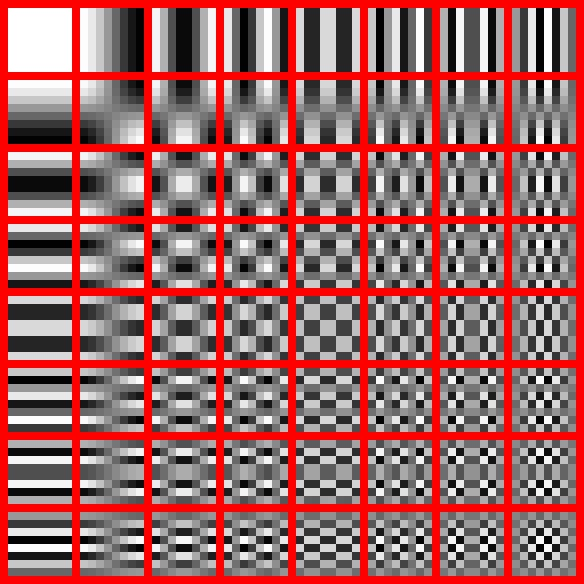
\includegraphics[width=4cm]{fig_9_9.jpg} 
	\caption{DCT basis.}\label{fig_9_9}
\end{figure}
\begin{figure}[h] 
	\centering 
	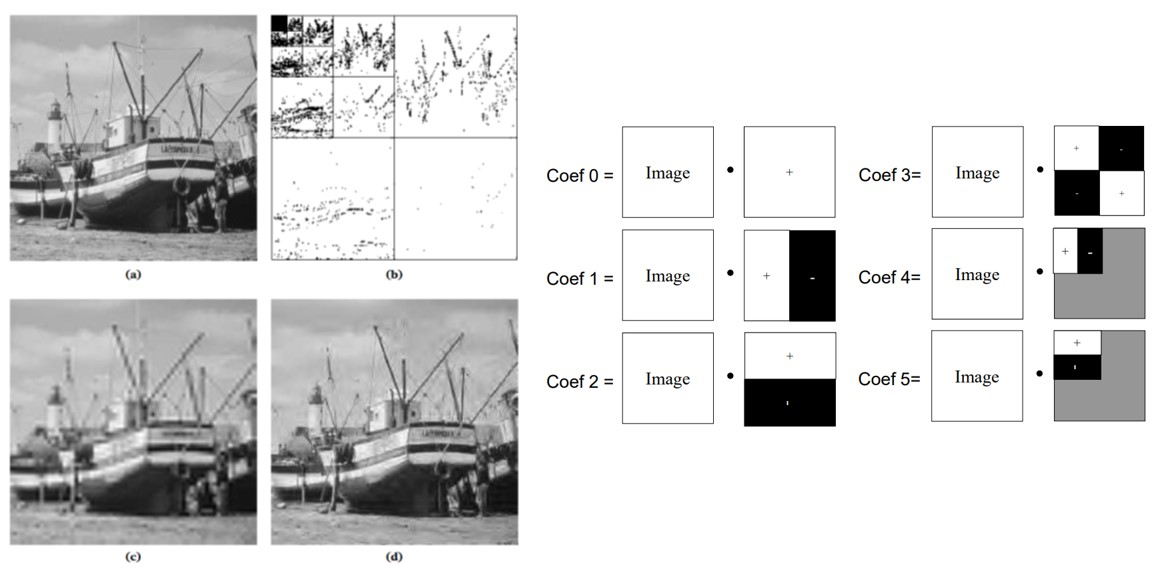
\includegraphics[width=12.5cm]{fig_9_10.jpg} 
	\caption{(Left) Image compression with wavelets: (a) Discrete image of $256^2$ pixels; (b) orthonormal wavelet coefficients at 4 different scales with black points correspond to large coefficients; (c) Approximation using the three largest scales; (d) Approximation using the $K$ largest coefficients ($K=\frac{256^2}{16}$). (Right) Definition of the first few (coarsest scale) wavelet coefficients of an image.}\label{fig_9_10}
\end{figure}
\begin{figure}[h] 
	\centering 
	\includegraphics[width=10cm]{fig_9_2D_wavelet.jpg} 
	\caption{Illustration of how the wavelet coefficients are arranged to form a pyramid. Left: each large block corresponds to a basis/filter and will be element-multiplied with the image to give an coefficient. Right: The way we arrange coefficients with different row/column frequencies to form the coefficient pyramid.}\label{fig_9_2D_wavelet}
\end{figure}
\par Wavelets turn out to be another successful way to compress images. Given an image shown in (a) of the left part of Figure \ref{fig_9_10}, we can compute the corresponding wavelet coefficients ((b) in the left of Figure \ref{fig_9_10}) and use them to construct approximations ((c) and (d)). The visualization of wavelets for images is often in this multiresolution representation. To understand this visualization, we can take a look at the right of Figure \ref{fig_9_10}\footnote{From https://www.cs.toronto.edu/~mangas/teaching/320/slides/CSC320L11.pdf
}. The first coefficient is just the average of all points corresponding to the most top-left block in (b). Then we apply the mother wavelet horizontally and vertically resulting in coefficients 1 to 3, corresponding to the 3 blocks (in the same size) around the top-left black block in (b). Then we do dilation and translation to generate more coefficients (Figure \ref{fig_9_2D_wavelet}). Note that as the basis function becoming more and more localized, it gains the ability to capture things with higher and higher frequency with, at the same time, larger and larger number of coefficients in the same scale (rearranging things gives the pyramid visualization results in (b)). (c) shows an approximation using only the coefficients in the three largest scales, which can be regarded as a low-pass filtering. In (d) we are more selective about where to keep the coefficients. Since most of parts in high-frequency coefficients are zeros, by throwing away small ones, we get a compression while keeping both the low-frequency properties as well as high-frequency things for important locations. Wavelets for its robustness with noise are also used for image denoising (for example see the slides).
\par Figure \ref{fig_9_11} shows an example for different compression algorithms. We see the mosaic-like things caused by DCT used in JPEG, while the wavelets produces better results with the same compression ratio. Note that wavelet other than Haar wavelet is used here.
\begin{figure}[h] 
	\centering 
	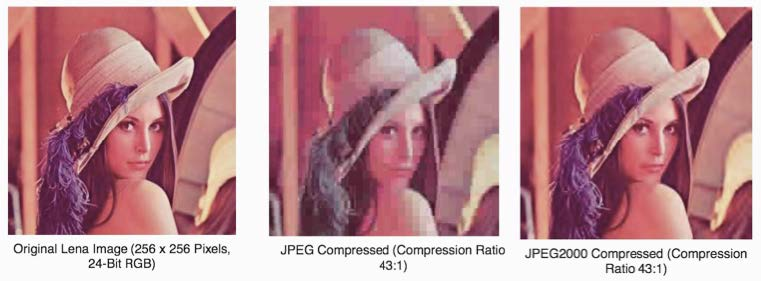
\includegraphics[width=12.5cm]{fig_9_11.jpg} 
	\caption{Results from different compression algorithms. JPEG: DCT; JPEG2000: wavelets.}\label{fig_9_11}
\end{figure}
One last thing to mention when it comes to image compression is the computational efficiency. Naively apply basis transformation ia matrix multiplication yield a $O(D^2)$ cost, where $D$ is the number of pixels in a image, and this can be gigantic. The way in practice we compute the transformation is not by explicitly instantiating the ${\bf U}$ matrix and doing multiplications, but by exploiting fast transforms:
\begin{itemize}
	\item Fourier: $O(D\log D)$
	\item Wavelet: $O(D)$ or $O(D\log D)$.
\end{itemize}
Another natural way to relieve this problem is by breaking up images into blocks, and transform each block. This avoids quadratic blow-up, but as shown in Figure \ref{fig_9_11} sacrifices perceptual qualities.
\section{Overcomplete Dictionaries}
In this section, however, we want to go beyond the orthonormal transforms and see how this can benefit sparsity representation. So far, based on the assumption that natural signals have approximate sparse representation in suitable orthonormal bases, e.g. wavelets for natural images, we have done a lot of things. Briefly speaking, in the coding via orthonormal transforms we do the following
\begin{itemize}
	\item given: signal ${\bf x}$ and orthonormal matrix ${\bf U}$
	\item compute linear transformation (change of basis) ${\bf z}-{\bf U}^T{\bf x}$
	\item truncate ``small'' values, ${\bf z}\mapsto \hat{\bf z}$
	\item compute inverse transform (recall ${\bf U}^{-1}={\bf U}^T$) $\hat{\bf x}={\bf U}\hat{\bf z}$.
\end{itemize}
The quality of reconstruction is measured by the error $\|{\bf x-}\hat{\bf x}\|^2$, and when we have a small error, we find a sparse coding vector $\hat{\bf z}$. Recall that for dictionary choice, the Fourier dictionary is good for ``sine like'' signals, while a wavelet dictionary is good for localized signals. As mentioned before, choosing a proper basis is hard in practice, so one natural thing to ask is why not just use a combination of these families of basis and just figure out which one is right after we have encoded the signal. This motivates the more general dictionaries we are going to talk about: overcomplete dictionaries. Actually, in terms of reconstruction, we don't need $>N$ atoms for signals in $\mathbb{R}^N$, but as we will see, in terms of sparsity, this setting is feasible and makes sense.
\par The idea of overcomplete dictionaries, motivated by that no single basis is optimally sparse for all signal classes, is really to exploit the overcompleteness (${\bf U}^{D\times L}$ such that $L>D$), which means we use more atoms (dictionary elements) than dimensions. Now the problem comes to how we can construct this dictionary, and with it how can we decode/reconstruct signals. Briefly speaking, we union orthonormal bases to generate overcomplete dictionaries, and use some coding algorithm to choose the best representation. Note that choosing the best representation is little bit more involved since by construction we can find multiple coding that can do the exact recovery due to the redundancy of representation.
\subsection{Encoding (Dictionaries)}
For constructing the dictionaries, the strategy is really to do it manually by signal inspection (looking at the signal and see what interesting properties does it have). We can simply try several and choose the one which affords the sparest coding. 
\par Here is one inspiring example from S. Mallat, A Wavelet Tour of Signal Processing – The Sparse Way, Academic Press, 2009. As shown in Figure \ref{fig_9_12}, signal might be a superposition of several characteristics, say smooth gradients and oscillating textures. Since a single orthonormal basis cannot sparsely code both, like wavelet basis might be good at the smooth gradient part while fails to captures the high-frequency texture part. The idea of building the dictionary is then to use algorithms to pick atoms (dictionary elements) from a union of bases, each one responsible for on characteristic.
\begin{figure}[h] 
	\centering 
	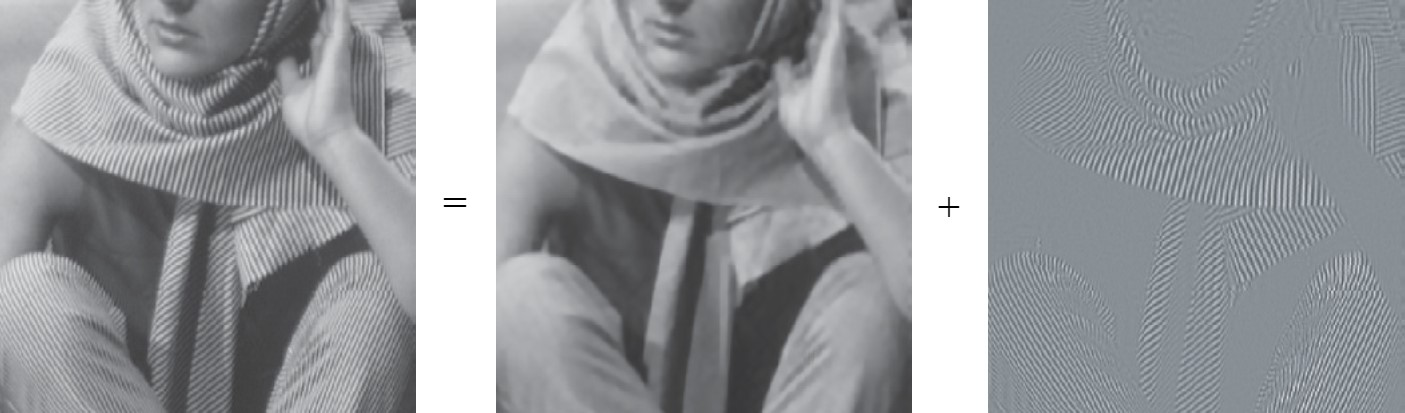
\includegraphics[width=12.5cm]{fig_9_12.jpg} 
	\caption{Signal might be a superposition of several characteristics.}\label{fig_9_12}
\end{figure}
\par As an example for capturing the oscillating texture, we introduce the following Gabor wavelets, which is directional oscillation with its amplitude modulated by a Gaussian window
\begin{align*}
g(n_1,n_2;\mu_1,\mu_2,f,\theta)&\propto \exp[-(n_1-\mu_1)^2]\exp[-(n_2-\mu_2)^2]\\
&\times\cos(f\cdot(n_1\cos \theta+n_2\sin\theta)).
\end{align*}
Figure \ref{fig_9_13} shows some examples of Gabor wavelets with different settings. The size of the dictionary size is determined by the discretizing parameter range of $\mu_1,\mu_2,f$ and $\theta$.
\begin{figure}[h] 
	\centering 
	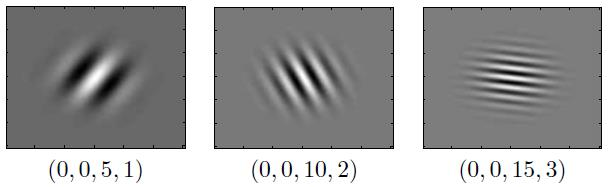
\includegraphics[width=12.5cm]{fig_9_13.jpg} 
	\caption{Examples of Gabor wavelets.}\label{fig_9_13}
\end{figure}
\par The following example gives some intuition about how general overcomplete dictionaries can benefit sparsity. Consider data set $\{{\bf x}_1,\dots,{\bf x}_{10000}\}\in \mathbb{R}^3$ as shown in Figure \ref{fig_9_14}, where data points mainly lie in 2 intersecting hyperplanes. (Actually I am not sure if this explains Figure \ref{fig_9_14}.)
\begin{figure}[h] 
	\centering 
	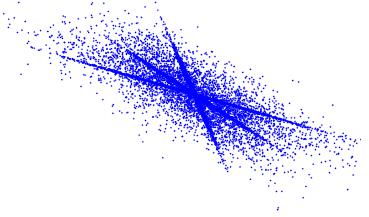
\includegraphics[width=5cm]{fig_9_14.jpg} 
	\caption{Visualization of the data set.}\label{fig_9_14}
\end{figure}
\par The full coding needs $(K=3)$ in spanning basis ${\bf U}\in \mathbb{R}^{3\times 3}$ to give accurate reconstruction. However, a $K=2$ coding with small error is possible using a four atom dictionary
\begin{equation*}
\tilde{\bf U}=[{\bf u}_1,{\bf u}_2,{\bf u}_3,{\bf u}_4]\in \mathbb{R}^{3\times 4},
\end{equation*}
where $[{\bf u}_1,{\bf u}_2]$ are the bases for the first hyperplane, while $[{\bf u}_3,{\bf u}_4]$ are the bases for the second hyperplane. 
\par Note that $L>D$ means the atoms are no longer linearly independent. We can define the overcompleteness by factor $\frac{L}{D}$, which also indicates the dictionary size. Increasing $\frac{L}{D}$ potentially increases the sparsity of the coding (we hope), while increases the linear dependency between atoms. If we have a very large $L/D$ there might even have several groups of atoms form the same subspace.
In this case we would like to have a way to measure the redundancy other than simply count the number of atoms by $\frac{L}{D}$. A way to do this is via a linear dependency measure for dictionaries: coherence, which is defined by 
\begin{equation*}
m({\bf U})=\max_{i,j:i\neq j}|{\bf u}_i^T{\bf u}_j|,
\end{equation*}
where we have $m({\bf B})=0$ for an orthonormal basis ${\bf B}$, and $m([{\bf B}\ {\bf u}])\geq \frac{1}{\sqrt{D}}$ if atom ${\bf u}$ is added to an orthonormal ${\bf B}$ (consider $1=\sum_i u_i^2\leq D u_{max}^2$).  
\subsection{Signal Reconstruction}
The main point to have this measurement comes from the hardness of finding the best/sparsest representation due to the redundancy in the dictionary. If we naively compute the coding ${\bf z}$ via ${\bf z} = {\bf U}^T{\bf x}$, 
for orthonormal ${\bf U}$ this is okay, we can simply compute ${\bf x}={\bf Uz}$. Even for cases that ${\bf U}$ is a spanning bases ($D$ linearly independent atoms), the reconstruction can be problematic, in a sense that in
\begin{equation*}
{\bf x} = ({\bf U}^T)^{-1}{\bf z},
\end{equation*}
inverting ${\bf U}^T$ can be ill-conditioned. To understand the word ``ill-conditioned'', considering the following example where
\begin{equation*}
{\bf U}^T=\frac{1}{2}\begin{bmatrix}
1&1\\
1+10^{-10}&1-10^{-10}
\end{bmatrix}
,\quad ({\bf U}^T)^{-1}=\begin{bmatrix}
1-10^{10}&10^{10}\\
1+10^{10}&-10^{10}
\end{bmatrix}.
\end{equation*}
This can be problematic, since a tiny distortion in ${\bf z}$ (caused by say some noise) will completely change the reconstructed ${\bf x}$ for the large elements in the inverse transform. For general dictionaries, where ${\bf U}\in\mathbb{R}^{D\times L}$ is overcomplete (L>D), finding the best representation ${\bf z}$ in terms of reconstruction error is ill-posed due to the redundancy in the dictionary. But if we say that the sparsity is the main thing that we care about, by adding a constraint: find the sparest ${\bf z}\in \mathbb{R}^L$ such that ${\bf x}={\bf Uz}$, the problem is now mathematically solvable. Formally, we now try to solve a problem given by
\begin{align}
\label{eq_9_L0}&{\bf z}^*\in\mathop{\arg\min}_{\bf z}\|{\bf z}\|_0\\
&{\rm s.t.}\quad {\bf x}={\bf Uz},\notag
\end{align}
where $\|{\bf z}\|_0$ counts the number of non-zero elements in ${\bf z}$. This means we want to find the sparest solution, under the equality constraint. However, this is in general a NP-hard combinatorial problem. To directly solve the problem, we can either try brute-force: exhaustive search over all atom subsets (exponential in $L$), or we can use some greedy approach, e.g. Matching Pursuit (Mallat \& Zhang 1993), which is to do the following:
\begin{itemize}
	\item assume (length) normalized atoms ${\bf u}_j$
	\item greedily select $j^*=\arg\max_j|\langle {\bf x},{\bf u}_j\rangle|$
	\item add $\hat{\bf x}\leftarrow \hat{\bf x} + \langle {\bf x},{\bf u}_{j^*}\rangle {\bf u}_{j^*}$, where $\hat{\bf x}$ is the reconstruction
	\item compute residual ${\bf x}\leftarrow {\bf x} - \langle {\bf x},{\bf u}_{j^*}\rangle {\bf u}_{j^*}$
	\item repeat until some condition is satisfied.
\end{itemize}
Note that just as many other greedy approach, matching pursuit has no guarantee to find the best representation in general. Another way that are better understood theoretically is to change the problem into a convex optimization task. Specifically, we change the objective from minimizing the $L_0$ norm to $L_1$ norm:
\begin{align}
\label{eq_9_L1}&{\bf z}^*\in\mathop{\arg\min}_{\bf z}\|{\bf z}\|_1\\
&{\rm s.t.}\quad {\bf x}={\bf Uz}.\notag
\end{align}
This convex optimization problem can be solved efficiently, and under suitable conditions on ${\bf U}$, the solution of the two problems are equivalent.
\subsection{Sparsity and Exact recovery}\label{sec_9_comp_sens}
We conclude this chapter with some supplementary materials from one of my favorite courses at ETH, Mathematics of Data Science by Prof. Afonso S. Bandeira. This subsection is again totally out of the scope of CIL, but since it is rather relevant I put it here. Feel free to skip!
\par Assuming that ${\bf x}$ has a sparse coding under a overcomplete dictionary ${\bf U}$, in order for (\ref{eq_9_L1}) to be a good procedure for sparse recovery (\ref{eq_9_L0}) we need two things:
\begin{enumerate}
	\item the solution of (\ref{eq_9_L1}) is meaningful for (\ref{eq_9_L0}) (hopefully to be the same)
	\item the solution of (\ref{eq_9_L1}) can be efficiently found.
\end{enumerate}
We first take a look at the second one. Let $\bm{\omega}^+$ and $\bm{\omega}^-$ be the positive part and the symmetric negative part of ${\bf z}$, meaning that ${\bf z}=\bm{\omega}^+ - \bm{\omega}^-,\ \bm{\omega}^+\geq {\bf 0},\ \bm{\omega}^-\geq {\bf 0}$ and, for each $i$, either $\omega_i^+$ or $\omega_i^-$ is zero. In this case, we have
\begin{equation*}
\|{\bf z}\|_1=\sum_i \omega_i^+ + \omega_i^- = {\bf 1}^T(\bm{\omega}^+ + \bm{\omega}^-).
\end{equation*}
Then we consider a linear programming given by
\begin{align}
\label{eq_9_lp}\min_{\bm{\omega}^+ , \bm{\omega}^-}\ &{\bf 1}^T(\bm{\omega}^+ + \bm{\omega}^-)\\
{\rm s.t.}\ &{\bf U}(\bm{\omega}^+ - \bm{\omega}^-) = {\bf x}\notag\\
& \bm{\omega}^+\geq {\bf 0}\notag\\ 
&\bm{\omega}^-\geq {\bf 0}.\notag
\end{align}
The optimal solution of (\ref{eq_9_lp}) will satisfy that for each $i$, either $\omega_i^+$ or $\omega_i^-$ is zero since if it is not satisfied, we can reduce the part where both $\omega_i^+$ and $\omega_i^-$ are greater than 0 and decrease the objective. Therefore solving (\ref{eq_9_L1}) is equivalent to solve a linear programming (\ref{eq_9_lp}) which is efficiently solvable. 
\par For the first requirement, recall our assumption that ${\bf x}$ has a sparse coding ${\bf z}^*$. Formally we require ${\bf z}^*$ to be $s$-sparse, i.e. $\|{\bf z}^*\|_0\leq s$. Let's consider when will ${\bf z}^*$ fail to be the unique optimal solution for the $L_1$ minimization problem (\ref{eq_9_L1}).
\par Let $S={\rm supp}({\bf z}^*)$ (the support of ${\bf z}^*$, i.e. the set of indexes of non-zero entries) and $|S|=s$. If ${\bf z}^*$ is not the unique optimal solution for (\ref{eq_9_L1}), there exists a non-zero vector ${\bf v}$ such that ${\bf z^*+v}$ is an optimal solution. This means
\begin{equation*}
\|{\bf z^*+v}\|_1\leq \|{\bf z}^*\|_1,\text{ and }{\bf U(z^*+v)}={\bf x},
\end{equation*}
which means ${\bf Uv}=0$. Also,
\begin{equation*}
\|{\bf z}^*_S\|_1 = \|{\bf z}^*\|_1 \geq \|{\bf z^*+v}\|_1 = 	\|({\bf z^*+v})_S\|_1 + \|{\bf v}_{S^c}\|_1 \geq \|{\bf z}^*_S\|_1 - \|{\bf v}_S\|_1 + \|{\bf v}_{S^c}\|_1,
\end{equation*}
where the subscript $S$ means restricting elements to $S$. This means if ${\bf z}^*$ is not the unique optimal solution for the $L_1$ minimization problem, there must exist some non-zero vector ${\bf v}$ in the kernel of ${\bf U}$, such that $\|{\bf v}_S\|_1\geq \|{\bf v}_{S^c}\|_1$. Since that $|S|\ll L$, it is unlikely for ${\bf U}$ to have vectors in its nullspace that are so concentrated on such few entries. This motivates the following definition.
\begin{definition}[Null Space Property]
	Matrix ${\bf U}$ is said to satisfy the $s$-Null Space Property (${\bf U}\in s$-NSP) if, for all ${\bf v}$ in ${\rm ker}({\bf U})$ (the nullspace of ${\bf U}$) and all $|S|=s$, we have
	\begin{equation*}
	\|{\bf v}_{S}\|_1<\|{\bf v}_{S^c}\|_1.
	\end{equation*}
\end{definition}
We see that by construction, if our overcomplete dictionary matrix ${\bf U}$ satisfies the Null Space Property for $s$, then for a ${\bf x}$ with a $s$-sparse coding ${\bf z}^*$, ${\bf z}^*$ will be indeed the optimal solution to (\ref{eq_9_L1}), which means with ${\bf U}$ it finds the best coding for any signal with a $s$-sparse coding.
\par There are many other properties leading to the coincidence of the solution to the $L_1$ minimization problem and the $L_0$ problem. A particularly useful one is the Restricted Isometry Property (RIP) defined by
\begin{definition}[Restricted Isometry Property (RIP)]\label{def_9_RIP}
	An $m\times p$ matrix $U$ is said to satisfy the $(s,\delta)$-Restricted Isometry Property (RIP) if 
	\begin{equation*}
	(1-\delta)\|z\|^2\leq \|Uz\|^2\leq (1+\delta)\|z\|^2
	\end{equation*}
	holds for all $s$-sparse $z$.
\end{definition}
RIP describes the property of approximately preserving the length of sparse vectors. The following theorem connects RIP to our topic
\begin{theorem}\label{thm_9_RIP}
	Let $x=Uz^*$ where $z^*$ is an s-sparse vector. Assume that $U$ satisfies the RIP with $\delta_{2s}<\frac{1}{3}$, then the solution $z_0$ to the $L_1$ minimization problem
	\begin{equation*}
	min_z \|z\|_1,\ s.t.\ Uz=x=Uz^*
	\end{equation*}
	becomes $z^*$ exactly, i.e. $z_0=z^*$.
\end{theorem}
The point to introduce RIP is to give some insight about how coherence that measures the redundancy of dictionary ${\bf U}$ can affect our coding. Recall the definition of (worst-case) coherence
\begin{equation*}
\mu:=m({\bf U})=\max_{i\neq j}\|{\bf u}_i^T{\bf u}_j\|.
\end{equation*}
Given a dictionary ${\bf U}$ with unit-length atoms and worst-case coherence $\mu$, then it has been proved that ${\bf U}$ will satisfies $(s,\mu(s-1))$-RIP meaning that it will be $(s,\frac{1}{3})$-RIP for $s\leq \frac{1}{3\mu}$. By theorem \ref{thm_9_RIP}, when $s\leq \frac{1}{3\mu}$, with dictionary ${\bf U}$ we can efficiently find the best sparse representation for all signals that for which there exists such $s$-sparse representation ${\bf z}^*$. This motivates the problem of designing dictionaries with smallest possible worst-case coherence. This is a central problem in Frame Theory.

\end{document}